%!TEX root = ../report.tex


%%%%%%%%%%%%%%%%%%%%%%%%%%%%%%%%%%%%%%%%%%%%%%
\chapter{Delanalyse 2: Forskellen på et delmarked og et segment er påvisningen af særegne (specifikke? partikulære) sociale processer indenfor delmarkedet \label{kapitel_delanalyse2_socialeprocesser}}
%%%%%%%%%%%%%%%%%%%%%%%%%%%%%%%%%%%%%%%%%%%%%%

Efter at have konstateret at der er en opdeling af arbejdsmarkedet for arbejdstagere i delmarkeder, hvor mobilitet indenfor delmarkederne er hyppig, og mellem delmarkederne sjælden, har dette kapitel til formål at svare på det andet forskningsspørgsmål:

\begin{tcolorbox}[title=Forskningspørgsmål,
subtitle style={boxrule=0.4pt} ]
  \tcbsubtitle{2.} Kan forskelle i de sociale processer vise, at der er tale om segmenter, og ikke blot delmarkeder?
\end{tcolorbox}

Dette forskningsspørgsmål vil jeg besvare ved at kigge på de sociale processer i delmarkederne.

Jeg vil vise, hvordan indkomst, køn og ledighed præger delmarkederne. Det vil jeg gøre først ved at kigge på arbejdsmarkedet på et overordnet plan, hvor jeg vil kigge på arbejdsmarkedet som helhed og vise spændvidden i forhold til indkomstniveau, kønsforskelle og ledighedsgrad.

Dernæst vil jeg fokusere på en række delmarkeder og kigge på, hvad der karakteriserer de forskellige delmarkeder i forhold til indkomst, køn, ledighedsgrad, uddannelse og mobilitet. Hvis der er forskelle i de sociale processer er det sandsynligt, at der er tale om segmenter, og ikke blot delmarkeder.


%%%%%%%%%%%%%%%%%%%%%%%%%%%%%%%%%%%%%%%%%%%%%%
\section{Indkomstniveau på delmarkederne \label{sec_delanalyse2_loen}}
%%%%%%%%%%%%%%%%%%%%%%%%%%%%%%%%%%%%%%%%%%%%%%

Indkomstfordelingen i den arbejdende del af den danske befolkning kan ses i \ref{delanalyse2_timelon_fordelingogfigur}. Vi kan se at indkomstfordelingen er nogenlunde centreret omkring gennemsnittet og medianen, hvilket også kommer til udtryk i standardafvigelsen på 76 kr/t. Det ses at fra > 250 kr/t falder antallet af personer ganske drastisk, hvilket også kan aflæses i percentilerne. Den “lange hale” af meget høje lønninger er ikke mange forundt, men det er tydeligt, at de, der så tjener over den 90. percentil, tjener eksponentielt mere og mere frem mod den højest (beregnede) timeløn på 2.155 kr. Det lave antal observationer skyldes at dette ikke er beregnet ud fra \texttt{DISCO}-grupperne, men ud fra antallet af personer: Det vil sige, at gennemsnittet er afhængigt af om vedkommende har været på arbejdsmarkedet.

\begin{figure}
\parbox[H]{8cm}{\null
  % \centering
  \captionof{figure}{indkomstfordeling i analyseudvalget, farvelagt efter udvalgte percentiler}
  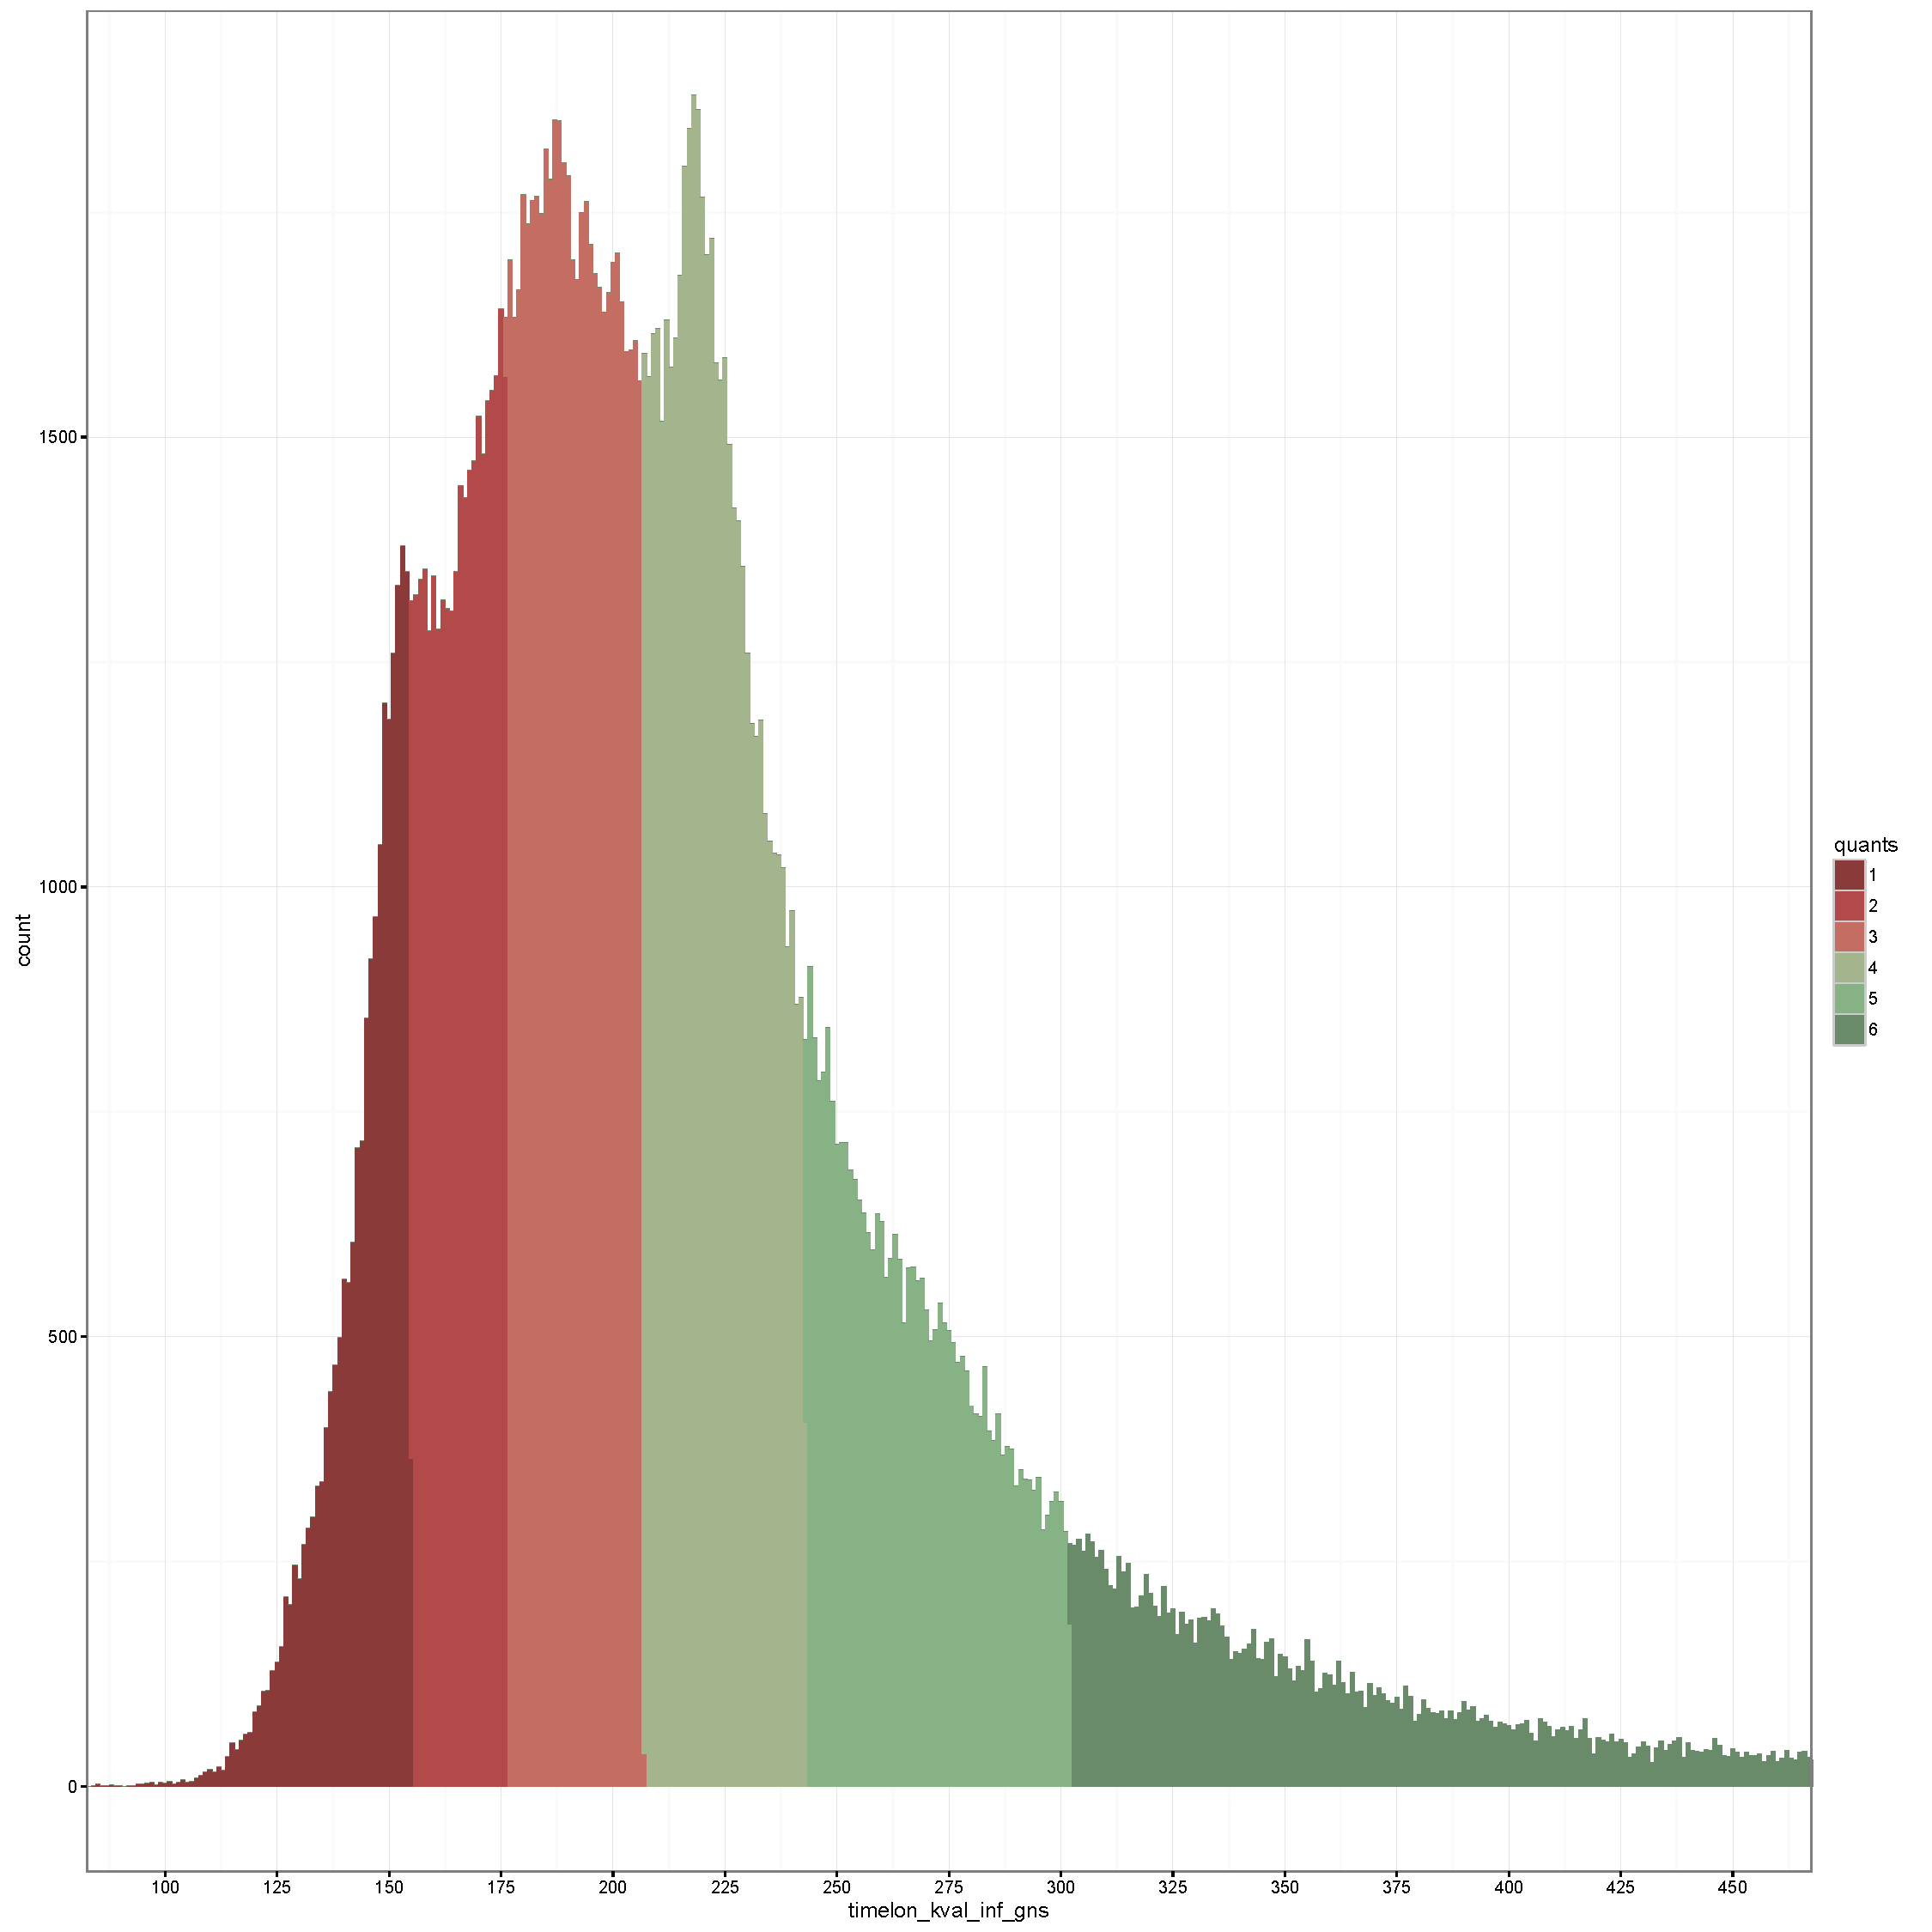
\includegraphics[width=7cm]{fig/deskriptive/timelon_quants.pdf}
}
\parbox[H]{5cm}{\null
\centering
  % \vskip-\abovecaptionskip
  \captionof{table}[t]{Udvalgte mål for indkomstfordelingen \label{delanalyse2_timelon_fordelingogfigur}}%
  \vskip\abovecaptionskip
%
% Table generated by Excel2LaTeX from sheet 'delanalyse2_indkomstfordeling'
\begin{tabular}{lr}
\toprule
Gennemsnit &                    222 kr.  \\
Sd-afvigelse &                      76 kr.  \\
\midrule
Mindste værdi &                      18 kr.  \\
Højeste værdi &                 2.155 kr.  \\
\midrule
10. percentil &                    155 kr.  \\
25. percentil &                    177 kr.  \\
Median &                    207 kr.  \\
75. percentil &                    243 kr.  \\
90. percentil &                    302 kr.  \\
\midrule
\textit{n} & \textit{205.798} \\
\bottomrule
\end{tabular}%

%
}
\end{figure}
%
Vi skal nu kigge nærmere på differentieringen i timeløn, og se, om de i kapitel \ref{delanalyse1_segmenteringsprocessen} fundne delmarkeder kan fortælle os noget om løndiffentieringener på arbejdsmarkedet. Når vi kigger på de 51 delmarkeder, som de fremgår af figur \ref{fig_analyse_deskriptivt_kort_timelon}, kan vi se lønforskelle mellem forskellige delmarkeder.

Lønforskellene fremstår tydeligt ved, at de hvide farver markerer medianen på 211 kr/time. De røde farver er under 211 kr/time. Jo mørkere rød, desto lavere timeløn. De grønne farver er over 211/time. Jo mørkere grøn, desto højere timeløn.

\newgeometry{left=-0.01cm,bottom=0.1cm}
\begin{figure}[H]
\begin{center}
  \caption{Intern mobilitet for klyngerne.}
  \label{fig_analyse_deskriptivt_kort_timelon}
  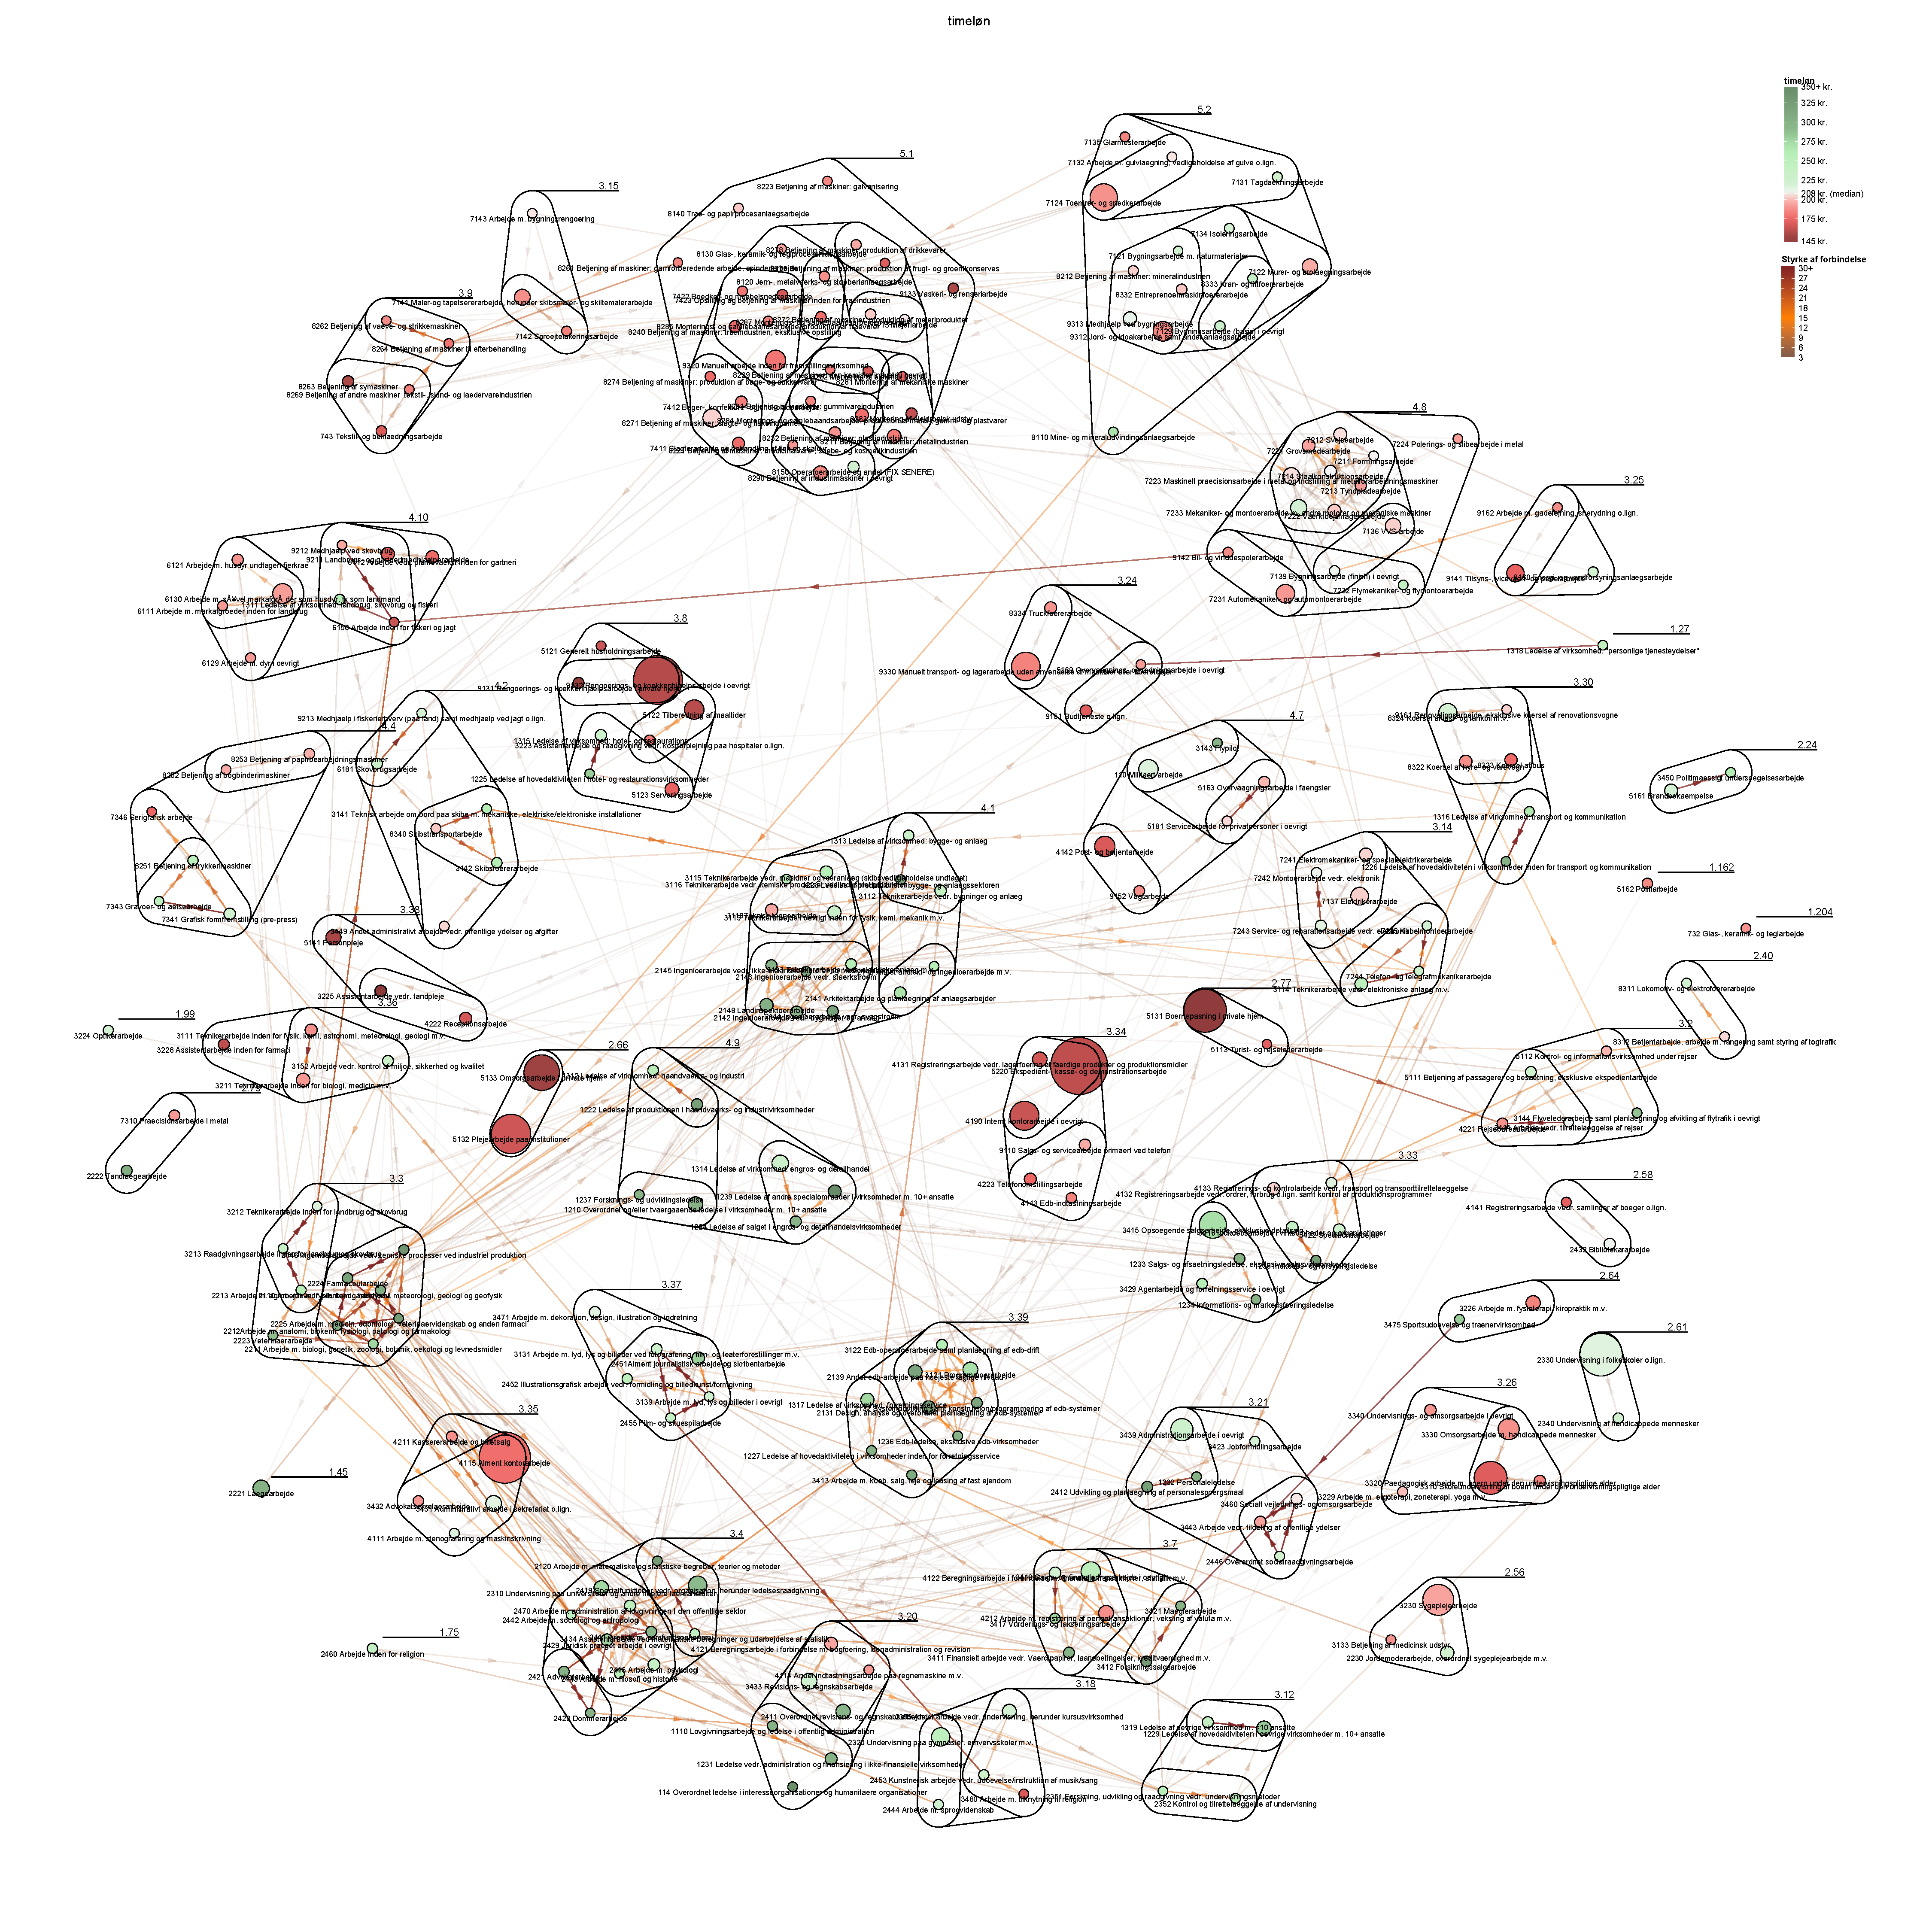
\includegraphics[width=1.0\textwidth]{fig/netvaerkskort/kort_timelon.pdf}
  \centerline{ \tiny{Kilde: Nielsen-Gravholt og Begtrup-Bright}}
\end{center}
\end{figure}
\restoregeometry

Hvilke delmarkeder har en høj timeløn og hvilke delmarkeder har en lav timeløn. For at illustrerer dette vil jeg zoomer ind på to delmarkeder. Det ene delmarked jeg vil fremhæve er delmarked \emak{s5.1}, som består af jobfunktioner relateret til primært faglært maskin- og fabriksarbejde herunder produktioner af mad, træ og metal. Det andet delmarked jeg vil fremhæve er delmarked \emak{s3.4}, som består af jobfunktioner relateret til akademisk arbejder herunder samfundsvidenskabeligt og humanistisk arbejde.
%
\begin{wrapfigure}{r}{6cm}
  \vspace{-20pt}
  \begin{center}
    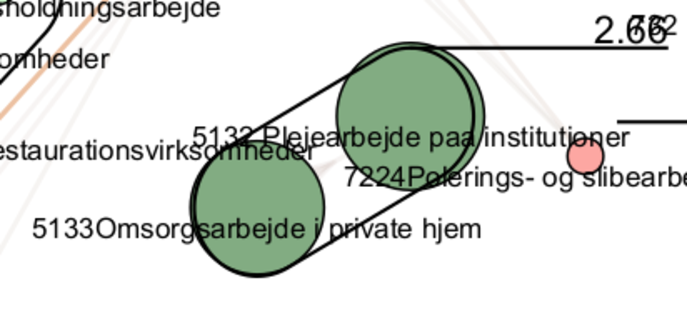
\includegraphics[width=6cm]{fig/segzoom/seg_2_66.pdf}
   \caption{}
   \label{fig_delanalyse1_zoom_2_66}
  \end{center}
  \vspace{-20pt}
\end{wrapfigure}
%
De personer som arbejder og skifte job inden for delmarked \emak{s3.4} arbejder som advokater, dommere, sociologer, antropologer, statistikere, undervisere på universitetere, historikere, filosoffer, psykologer. De får en løn som i gennemsnit spænder fra XXX kr/time for de laveste (hvem er det) til XXX kr/time (hver er det). Udover en høj timeløn har de det til fælles at det typisk kræver en lang videregående uddannelser for at besidde disse job. Nogle jobs såsom advokat- og dommerarbejde har kræver udover en lang videregående uddannelser og en særlig efteruddannelse.
%
\begin{wrapfigure}{r}{6cm}
  \vspace{-20pt}
  \begin{center}
    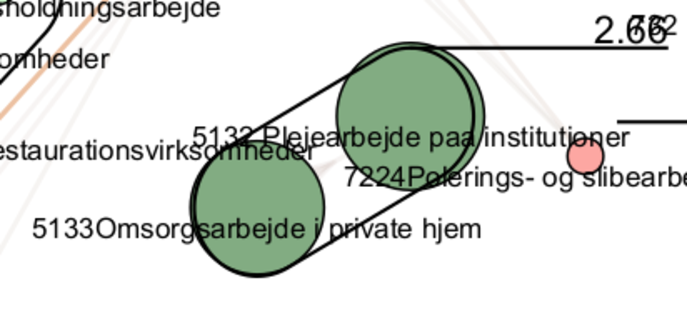
\includegraphics[width=6cm]{fig/segzoom/seg_2_66.pdf}
   \caption{}
   \label{fig_delanalyse1_zoom_2_66}
  \end{center}
  \vspace{-20pt}
\end{wrapfigure}
%
De personer som arbejder og skifte job inden for delmarked \emak{s5.1} arbejder som slagtere, bagere, mejerister, arbejde med betjening af maskiner, monteringsarbejde, samlebåndsarbejde og manuelt arbejde. De får en løn som i gennemsnit spænder fra XXX kr/time for de laveste (hvem er det) til XXX kr/time (hver er det) med en enkelt afstikker på XXX kr/time. Udover en lavere timeløn har de det til fælles at det typisk kræver en erhvervsuddannelse eller et kortere kursus at besidde disse job.

Den første umiddelbare umiddelbare forklaring på lønsforskellen mellem de to segmenter er uddannelse. For at arbejde inden for de to delmarkeder kræver det en uddannelse. Forskellen er så længden på uddannelsen. Det er anerkendt, at der er en sammenhæng mellem uddannelse er løn. Human kapital er en økonomisk teori udviklet af Gary Becker, der beskriver, at arbejdstagere kan tage en uddannelse som en investering mod forventning om økonomisk kompensation ved at vedkommendes produktivitet øges (fx Cahub og Zylberberg 2004, s. 69). Da de akademiske uddannelser tager længere tid end erhvervsuddannelser og kortere kursus, giver det også en højere økonomisk kompensation. 


%%%%%%%%%%%%%%%%%%%%%%%%%%%%%%%%%%%%%%%%%%%%%%
\newpage \section{Kønsforskelle blandt delmarkederne \label{sec_delanalyse2_loen}}
%%%%%%%%%%%%%%%%%%%%%%%%%%%%%%%%%%%%%%%%%%%%%%


\iffalse
\label{iffalse}

Attributterne er ikke anvendt som inklusionskriterier og kan derfor bruges til at
vurdere, hvorvidt der er overensstemmelse mellem privilegerede positioner i netvær-
ket og symbolske eller økonomiske privilegier, der er eksterne for netværket. Dette giver
os mulighed for at vurdere om vores specifikation af netværket stemmer overens med
magtsymboler, hvilket kan benyttes til at vurdere validitet ( 1983, s. 29).


validitet i et klasseskema: ekstern og intern validitet (Oesch s. 94)

indkomst som udtryk for magt på arbejdsmarkedet og social status. Dermed "den afgørende faktor" for menneskers livschancer. s. 95

Boje peger på faren ved at fokusere på outcomet af sociale processer såsom lønforskelle, arbejdsløshed, hyppige jobskifte m.m.. Det er en reel fare ved mit empiriske arbejde. s. 28, men meget god hvis man vil sikre sig at alt er, som det skal være. 

Grundet den danske struktur og fokus på organisering må det forventes, at mobilitets- og lønbarrierer primært findes indenfor fag, og ikke indenfor industrier/erhvervsgrene, hvilket findes i USAs langt mindre organiserede og mere monopolitiske virksomhedskultur. 

"i perioder med økonomisk tilbagegang og hvor der på arbejsmarkedet er overudbud af lønarbejdere synes barriererne mellem segmenterne at blive skærpet." (...) og nye segmenter og delmarkeder opstår på den baggrund. s. 72
→ perioden 1996-2009 er en periode med vækst, dvs: Det her en god periode. Find tal for økonomisk vækst for perioden


brug relative forskel mellem lønninger, ikke bare den absolutte, som må siges at være den vigtigste for personerne selv. Brug medianen for den "nederste klasse" som udtryk for lønniveauet. Kan du overføre det til dit eget? lønniveauet for den lavest tjenende klynge?

Oesch afviser at "future prospects" skulle have stor betydning, da han mener at påvise en stærk sammenhæng mellem nuværende lønninger og fremtid indkomst. I danmark, viser Esping-Andersen, fungerer low-income jobs sådan. Men vi kan jo se, hvor folk bevæger sig hen. Og det ser ikke ud til at være en stærk sammenhæng mellem service-jobs og future prospects. Undersøg servicejobs og ande


find ud af hvor mange skift der er per år. Dejligt konkret tal. henvis til boje 1988 s. 123


Løndannelsen s. 79-80
	i det sekundære arbejdsmarked synes der ikke at være en sammenhæng mellem løn og uddannelse - det er ikke det, der er det centrale. Hvorimod på det primære arbejdsmarked synes det netop at være betydningsfuldt, her er uddannelsesmæssige ressource nøje afstemt med løn. 
	tre forhold spiller ind:
	- institutionel regulering kontra markedsregulering: I DK er stort set al løndannelse reguleret gennem institutionelle aftaler 
	→ har nok ændret sig noget siden, men i det store og hele nok stadig rigtigt
	- Lønnen knyttet til job kontra til præstation.
	- lønnen tilnyttet stillingsmæssigt avancement/ikkeavancement. primære forskel på sekundær/primær løn. det sekundære jobmarked har samme lønninger livet igennem. 





















% %%%%%%%%%%%%%%%%%%%%%%%%%%%%%%%%%%%%%%%%%%%%%%
% \section{kønsforskelle i sociale processer \label{sec_delanalyse2_køn}}
% %%%%%%%%%%%%%%%%%%%%%%%%%%%%%%%%%%%%%%%%%%%%%%

% En grundlæggende differentieringsform i snart sagt alle samfund er



%  kønsopdelingen, der kommer til udtryk i en kønsbestemt arbejdsdeling i langt de fleste samfund. Som David Oesch bemærker, er det påfaldende, hvor få kvantitative undersøgelser af arbejdsmarkedsrelationer, der inddrager køn i analyserne  














\fi


